\section{Observation}


% During the prefill stage, efficient KV cache compression often relies on an input-side observation window to estimate token importance. However, these static, prompt-centric windows are inherently misaligned with the dynamic queries of the actual decoding process. Consequently, they frequently fail to capture the true attention distribution that generation context concerns, leading to the erroneous eviction of critical  tokens. And ground-truth decoding queries are inherently unavailable during inference, rendering them impractical for directly guiding eviction. 

Given the discussion in Section \ref{sec:introduction}, constructing pseudo queries to accurately approximate the unavailable ground-truth decoding queries becomes crucial. Building upon CaliDrop's \citep{calidrop} insight that queries at adjacent positions exhibit high similarity, we hypothesize that this similarity is strongly correlated with positional information rather than semantic content. This prompts us to investigate whether positional information alone can effectively approximate future decoding queries without relying on true decoding content. See Appendix \ref{Preliminary Experiment Details} for details of preliminary experiments.
% Preliminary experiments confirm that positional information plays a more critical role than contextual content in approximating decoding-stage queries, providing a robust foundation for our the position-aware pseudo-query approach.

% \begin{figure*}
    \centering
    % 第一张子图及图注
    \begin{subfigure}[t]{0.47\textwidth}
        \centering
        \resizebox{\textwidth}{!}{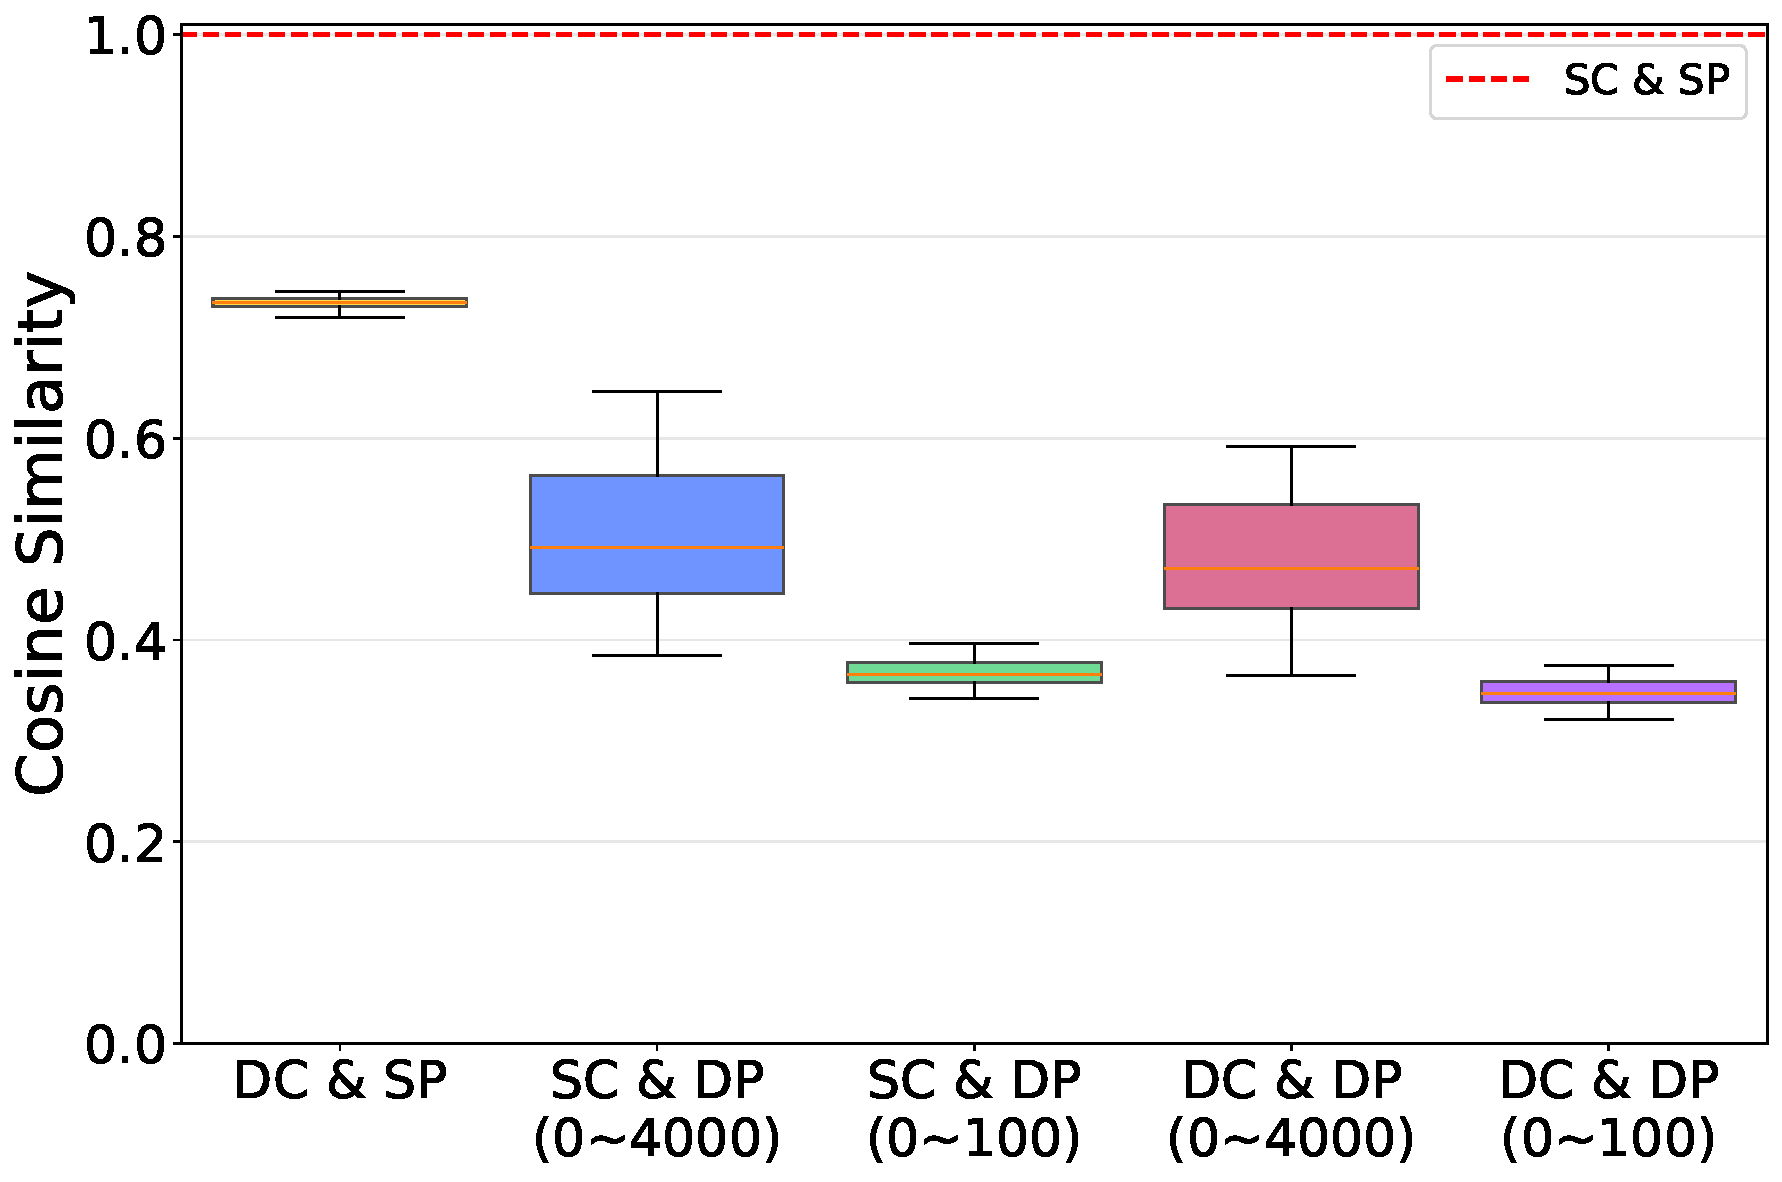
\includegraphics{images/similarity_boxplot.pdf}}
        % \caption{Boxplot of query similarity distributions.}  % 第一张图的图注
        \caption{}  % 第一张图的图注
        \label{fig:query_similarity_boxplot}
    \end{subfigure}
    \hspace{0.5cm}  % 两图间距
    % 第二张子图及图注
    \begin{subfigure}[t]{0.47\textwidth}
        \centering
        \resizebox{\textwidth}{!}{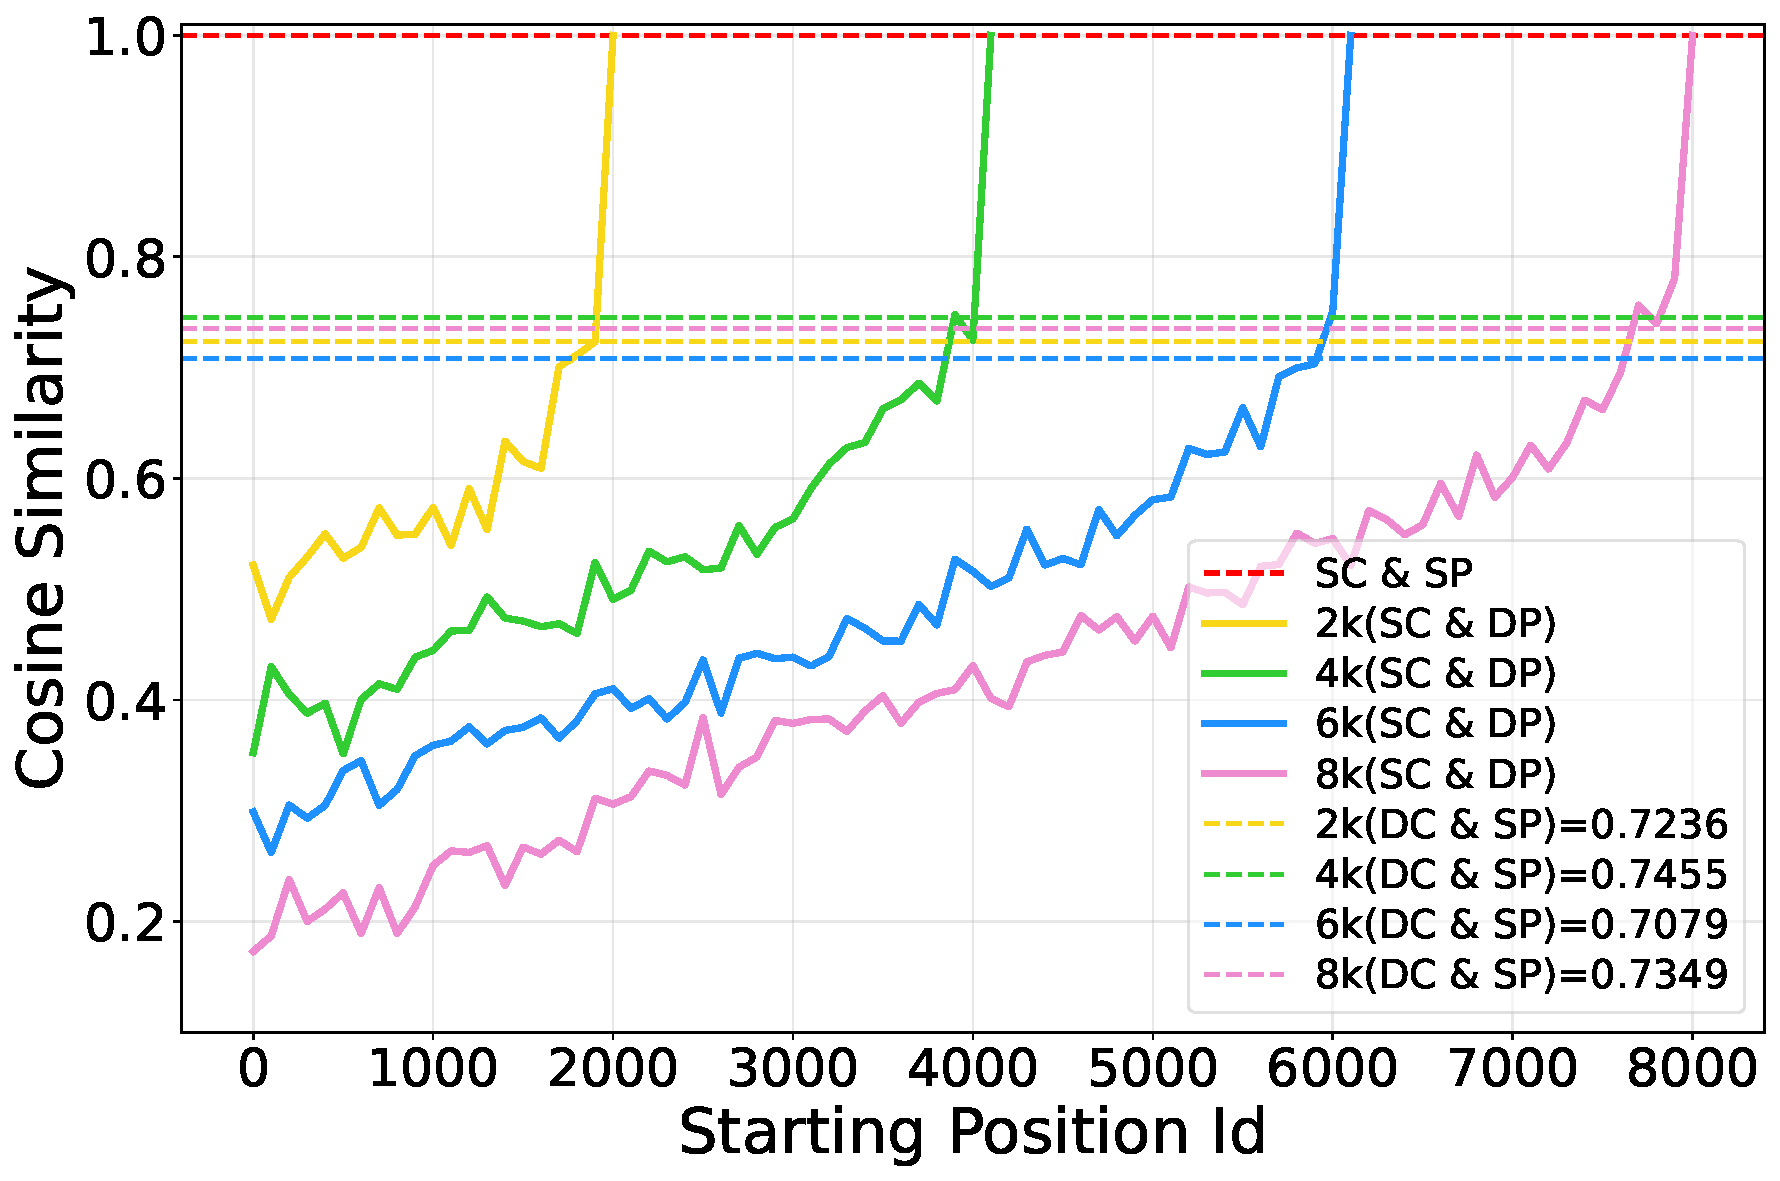
\includegraphics{images/average_similarity_curve.pdf}}
        % \caption{Curve of query similarity over offset positions.}  % 第二张图的图注
        \caption{}
        \label{fig:query_similarity_curve}
    \end{subfigure}
    \vspace{-7pt}
    % 可选总标题（概括两图内容）
    \caption{Analysis of Positional Dominance and Offset Sensitivity in Query Similarity. We set the pseudo queries of fixed length 32. (a) Boxplot of query similarity distributions for a 4k context under different content and position conditions, each aggregated from 100 independent trials. DC: pseudo-queries content is constructed by randomly sampling 32 tokens from the model's vocabulary; DP: pseudo-queries positions are assigned by randomly sampling a consecutive span of 32 index positions from the context length range [0, m] (e.g., [0, 4000]). (b) Query similarity curves over offset positions for contexts of lengths 2k, 4k, 6k, and 8k. The x-axis denotes the starting position assigned to pseudo queries (e.g., an x-axis value of 3500 corresponds to position IDs $3500\sim3531$).}
    % \caption{Analysis of Positional Dominance and Offset Sensitivity in Query Similarity. (a) Query similarity distributions from large-scale sampling of content and position variations. DC: pseudo-queries content is constructed by randomly sampling 32 tokens from tokenizer's vocabulary; DP: pseudo-queries positions are assigned by randomly sampling consecutive span of 32 indices from [0, m]. (b) Similarity decay with positional offset across context lengths(2k-8k). Similarity decay with positional offset across context lengths.We sample instances from GovReport with input lengths of 2k, 4k, 6k, and 8k. The x-axis indicates the starting position of the 32-token pseudo-queries (e.g., 2500 corresponds to position IDs 2500–2531).  }

    \vspace{-14pt}
\end{figure*}

%Experiment select an example (input token length: 4424) from the GovReport dataset for summarization task. True queries comprise the first 32 output tokens from LLaMA-3-8B-Instruct with content \textcolor{gray}{"The report discusses the Federal Aviation Administration's (FAA) state block grant pilot program, which is part of its Airport Improvement Program (AIP). The program"} at positions \textcolor{gray}{4424-4455}. We artificially synthesized a 32-length context with \textcolor{gray}{"Sorry, I don't know. Sorry, I don't know. Sorry, I don't know. Sorry, I don't know. Sorry, I"}. Pseudo queries vary in both content (correct:\textcolor{gray}{"The report discusses..."} or incorrect: \textcolor{gray}{"Sorry, I don't know..."}) and position assignments (correct: \textcolor{gray}{4424-4455} or incorrect: \textcolor{gray}{0-31}). Results represent cosine similarity between pseudo queries and true queries under Post-ROPE and Re-ROPE conditions.


%\caption{Experimental setup using a GovReport summarization example (input length: 4424) with LLaMA-3-8B-Instruct. True queries comprise the first 32 output tokens with content \textcolor{gray}{"The report discusses the Federal Aviation Administration's (FAA) state block grant pilot program, which is part of its Airport Improvement Program (AIP). The program"} at positions \textcolor{gray}{4424-4455}，same as Table 1' experimental setting. Pseudo-queries use random token sequences from the tokenizer vocabulary as semantic content. Position assignments vary: correct positions (\textcolor{gray}{4424-4455}), wide-range incorrect positions (32 consecutive positions randomly selected from 0-4000), and narrow-range incorrect positions (32 consecutive positions from 0-100). Dashed lines indicate the specific SC&DP (0.3267) and DC&DP (0.3522) Post-ROPE similarity values from Table 1 for reference.}”.Each configuration was tested over 50 times with averaged results.Statistical results are based on 50 trials per configuration.

\subsection{Position Drives Query Representation}
% Our investigation reveals a pivotal insight: the semantic content of a query plays a secondary role compared to its positional encoding in determining its representation within the model's latent space. 
As detailed in Table \ref{table:query_similarity},We compare cosine similarities between ground-truth decoding queries and pseudo queries across four conditions: SC (Same Content), DC (Different Content), SP (Same Position), and DP (Different Position). Specifically, pseudo queries assigned correct future positional IDs but composed of completely irrelevant or nonsensical content (\textcolor{green}{DC\&SP}), exhibit strong cosine similarity (\textcolor{green}{0.7238}) to the actual target decoding queries. Conversely, queries with the identical semantic content but incorrect positional IDs (\textcolor{red}{SC\&DP} vs \textcolor{green}{SC\&SP}) fail to accurately approximate the target queries (\textcolor{red}{0.3522} vs \textcolor{green}{1.0000}). Notably, the comparison between DC\&SP and SC\&DP highlights that maintaining correct positional alignment achieves 2.1× higher similarity than maintaining correct content alone. The stark contrast underscores that the semantic content of queries plays a secondary role compared to positional encodings in constructing query approximations. The consistently high similarity under Pre-ROPE conditions (\textcolor{green}{0.7238} to \textcolor{green}{0.7913}) confirms that the model's underlying processing does not rely heavily on semantic content to distinguish between these query vectors, thereby underscoring that the dramatic disparity observed in Post-ROPE scores is almost attributable to the positional information. A large-scale statistical analysis (Figure \ref{fig:query_similarity_boxplot}) confirms the pervasiveness and consistency of the above phenomenon. 


% \subsection{Positional Offset Harms Similarity}
\subsection{Precise Positional Alignment is Necessary}
Building upon the dominance of positional information, we further quantify how the positional alignment of pseudo queries affects their similarities to true decoding queries. As shown in Figure \ref{fig:query_similarity_curve}, we fix the pseudo-query semantic content to match the true output and systematically vary their assigned positional IDs. \textbf{Results reveal a monotonic decay in the query similarity as the absolute offset increases between the assigned position and the correct position}. This decay phenomenon is consistently observed across diverse context lengths (2k to 8k), which is more pronounced in longer context scenarios. The strong sensitivity to positional misalignment underscores the critical dependence of query approximations on precise positional information. Consequently, accurately simulating decoding queries requires precise alignment with the future generation positional IDs.

\begin{figure}[htbp]
    \centering
    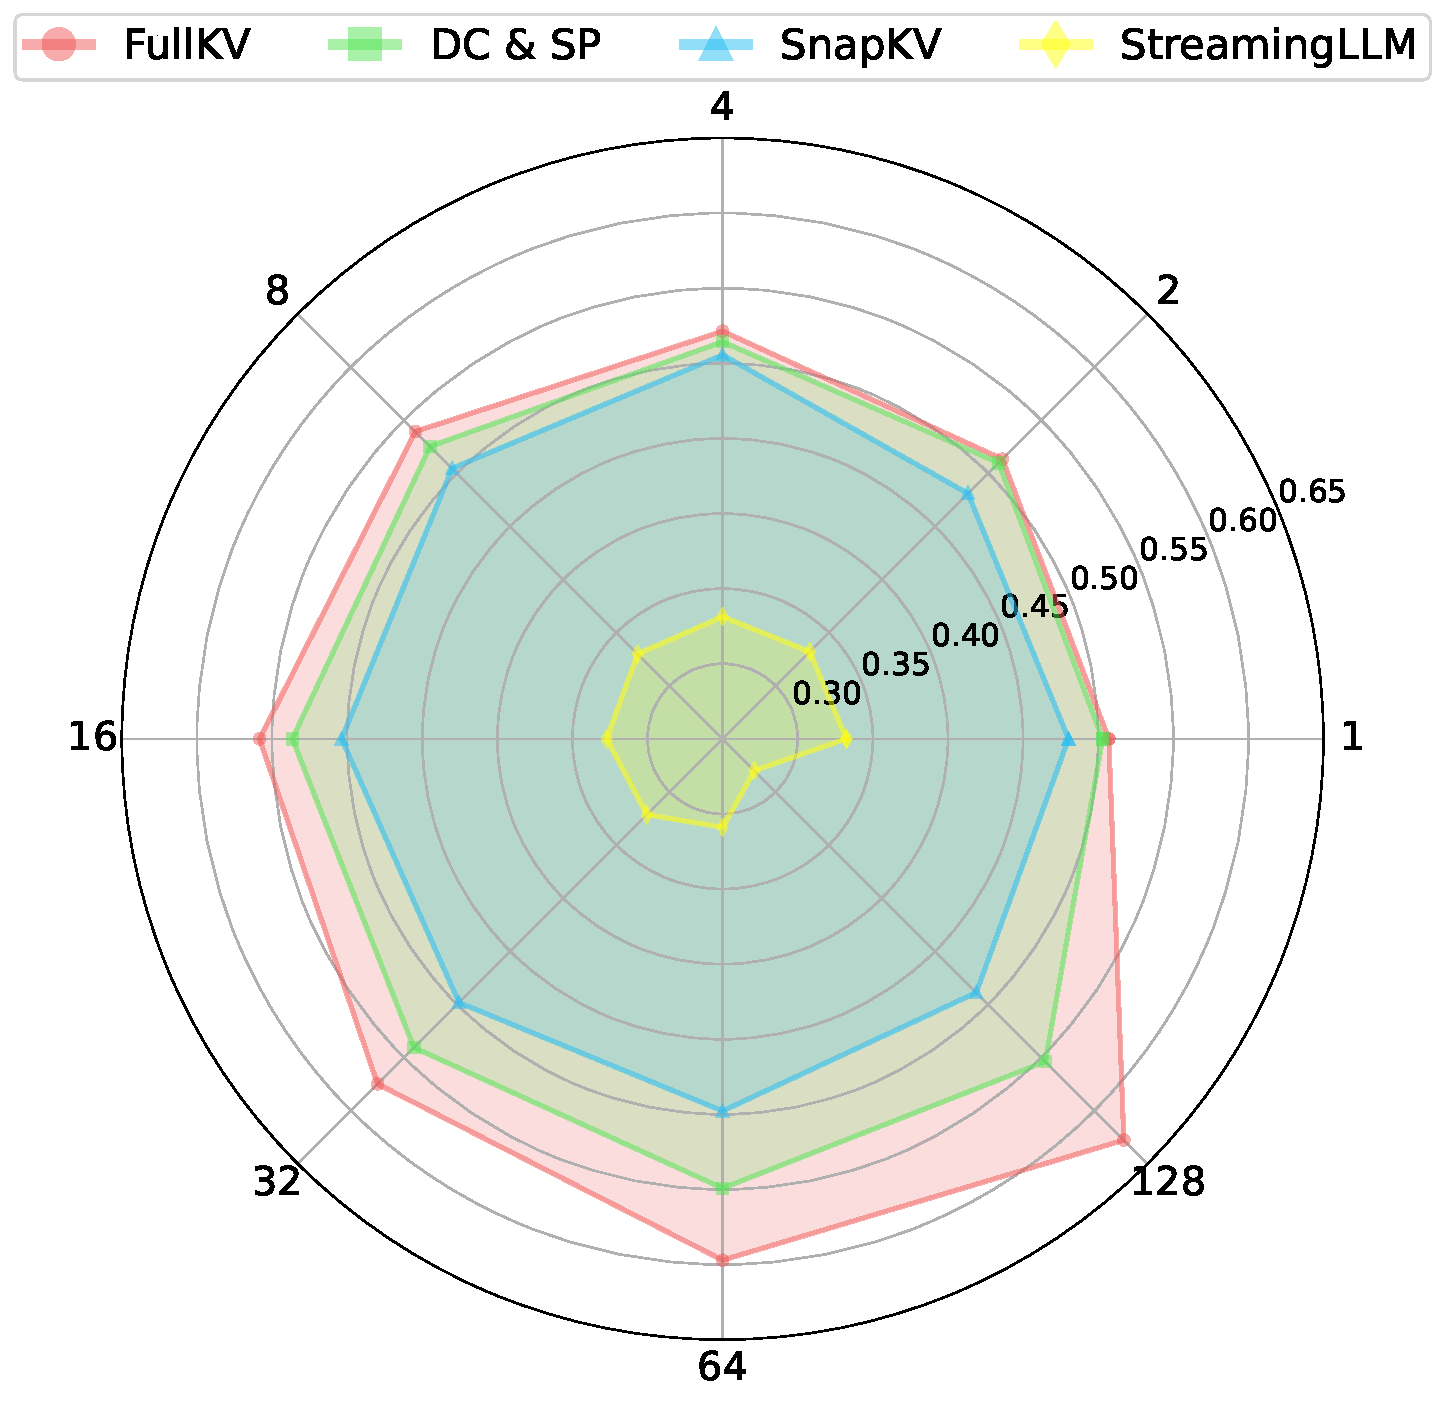
\includegraphics[width=\linewidth]{images/recall_radar_new_512.pdf} % 插入图片
    \vspace{-18pt}
    \caption{Recall Performance of different methods across various Window Sizes.} 
    \label{fig:recall_radar} % 图片标签（用于交叉引用，可选）
    \vspace{-18pt}
\end{figure}

\subsection{Position-Based Queries Enable More Accurate Token Eviction}
The critical question is whether higher query similarity translates into more accurate token eviction. To quantify this, we evaluate the recall of eviction strategies, which measures its ability to retain the tokens that are most important for the actual generation. Following the methodology of prior work \citep{lookahead}, the recall rate of the selected KV cache is defined as the proportion of indices selected by the observation window that overlap with those selected by all response tokens from the model. We define the recall metric as follows:


Let $R$ be the set of all tokens in the ground-truth response, and let $K$ be the full key cache from the prefill stage. The gold standard set of indices $M_{\text{gold}}$ for a given budget $B$ is determined by accumulated attention scores from all true response queries:
\begin{equation}
M_{gold} = \underset{{i \in [0, N)}}{TopK}\left( \sum_{j \in R} \text{Attention}(q_j, K) \right),
\end{equation}
where $N$ is the number of all prefill tokens, and $TopK$ returns the indices of the tokens with the highest accumulated scores. The predicted set of indices $M_{\text{pred}}$ is defined analogously to $M_{\text{gold}}$, but computed using only the queries in a candidate observation window $W$:
\begin{equation}
M_{pred} = \underset{{i \in [0, N)}}{TopK}\left( \sum_{j \in W} \text{Attention}(q_j, K) \right).
\end{equation}

The recall is the proportion of the gold-standard tokens that are correctly retained:


\begin{equation}
Recall_{W} = \frac{| M_{\text{gold}} \cap M_{pred} |}{| M_{gold} |}.
\end{equation}


We evaluate this recall metric on the GovReport dataset for different observation windows. As shown in Figure \ref{fig:recall_radar}, the window composed of pseudo queries with randomized content but correct future positions achieves significantly better recall than baselines like SnapKV and StreamingLLM. Notably, it maintains high recall even as the window size is reduced to 32 or 16, showing the high effectiveness and accuracy of position-based estimation. This demonstrates that a small set of pseudo queries, informed solely by precise positional forecasting, provides a highly effective basis for importance assessment, enabling accurate eviction even under extreme window constraints.


In summary, our experiments converge on a pivotal insight: the representation of a query vector is dominated by its positional encoding, with semantic content playing a secondary role. From the perspective of query-key interactions, this further implies that the attention pattern relies heavily on positional information to establish importance distribution, while exhibiting considerable robustness to variations in semantic content. This leads to a profound practical implication: high-fidelity decoding pseudo queries can be synthesized from positional encodings, entirely bypassing the computationally expensive and memory-intensive process of token generation. This position-aware query approximation forms the foundation of our method.





% 太直白了，得过渡一下，不能一上来就，为了探索更effective的window，你得简单说一下，以前的window怎么怎么样，为什么不好，等等，然后才说我们想要探索一个什么样的window。然后也不能一上来就，我们做了什么什么实验，发现什么事情，你得先引导读者， 你是怎么想的，然后你为什么会想到要做这个实验，你做这个实验是为了验证什么（你的假设是什么），然后这个实验有什么样的结果，最后ok，印证了我们的假设，表明了我们的window更好/更efficient/更effective。
%比如，这里可以，我们在previous的work中发现，相邻的query很相似，那么是否有可能query的相似度和position是有很大关联的，于是我们是否可以在不知道未来context是什么样的情况下通过position去做近似？然后发现position是更重要的，而非query。
% 简单来说就是，我们想要estimate未来的query，那如何预测呢？我们从以前的work中发现。。。，这种现象引发我们进一步探索/挖掘position与query相似度的关系，挖掘这种现象源于何处（rope）？这种性质是否可以为我们所用（our method）？
% ？这是什么翻译过来的？读不懂。另外，这个小节和上面一个小节想论述的不是一个东西吗？
% 这一段思路是ok的，打磨一下细节，公式的符号等，例如Top-B要改TopK, 没见过用Top-B的。就算与attention的K重了也没关系。

